\documentclass{beamer}
\usepackage{graphicx}

\usepackage{subfigure}

\usepackage{amsmath}
\usepackage{amssymb}

\usepackage{ulem}

\usepackage{url}

\usepackage{tikz}
\usetikzlibrary{calc,positioning,graphs,shapes,quotes,arrows}
\usepackage{ctex}
\usepackage{pgfplots}
\pgfplotsset{width=10cm,compat=1.9}

\usepackage{hyperref}
\hypersetup{hidelinks,
      colorlinks=true,
      allcolors=blue,
      pdfstartview=Fit,
      breaklinks=true}

\usepackage[backend=bibtex,sorting=none]{biblatex}
\addbibresource{Finalhw.bib}
\setbeamerfont{footnote}{size=\tiny}

\setlength{\parindent}{2em}
\usetheme{AnnArbor}
\usecolortheme{beaver}
\usefonttheme{default}
\setbeamertemplate{bibliography item}[text]

%---

\title{一维非线性方程的求根}
\author{南子谦 3210104676}
\institute{信息与计算科学}
\date{\today}
\begin{document}
\begin{frame} 
\titlepage
\end{frame}

%---

\begin{frame}
\frametitle{摘要}
\ 未知数和一些常数不仅施行有限次代数运算,而且还要施行有限次指数、对数、三角函数等运算,这样的方程叫做超越方程。对于一般的超越方程,没有求根公式可以使用。
对于代数方程,当次数大于5时无精确的求根公式。而实际问题中,欲求得方程的根时,不一定要得到根的准确值,而只需求得满足一定精度的近似值即可。本文章主要介绍求解近似根的各种方法。
\par 方程求根问题包括三个问题,根的存在性,有根区间的确定和根的精确化。只要确定出若干个区间,使得每个区间内y=f(x)与x轴有且只有一个交点,再根据特定算法逼近根即可。
\end{frame}

%---

\begin{frame}
\frametitle{引言}
随着科学技术的高速发展,非线性科学的应用已经涉及各个行业,例如气
象资料分析、飞机,汽车及轮船的设计、石油地质、计算生物化学、航天航空
领域和轨道设计、信息化援救等方面有着大量的实际问题,这些问题都要借助
于非线性模型来描述,最终都可以归结为非线性方程和非线性方程组的求解问
题。而对于次数大于 4 次的代数方程,它的精确解已经不能用解析方法求出,
这时想要求出方程的近似解只能寻求某种数值方法,而非线性方程组的求解要
更加困难。所以,无论在理论意义还是在实际应用中,运用数值方法求解非线
性方程和非线性方程组都是非常重要的。
\end{frame}

%---

\begin{frame}
    \frametitle{数学理论}
    \framesubtitle{定义}
    (连续)设函数$F:D \subset R^n \rightarrow R^n$,若对$\forall \xi>0$, $\exists \delta>0$,使得对任意的$x \in S(x_0,\delta)$
    =${\left|x-x_0 \right|<\delta}\subset D$都有
    \begin{equation}
    \left|F(x)-F(x_0)\right| < \xi
    \end{equation}
则称$F(x)$在点$x_0 \in int(D)$,若$F(x)$在D内每一点连续,则称$F(X)$在D内连续。
\end{frame}

\begin{frame}
    (迭代法的定义)现在给定一个初始点$z_0$或者几个初始近似值$z_0,z_1,z_2,\cdots,z_r,\cdot$,其中r为有限个,同时保证r 为正整数,可以依据某种格式产生一个有限或者无限序列
    \begin{equation}
        x_0,x_1,x_2,\cdots,x_n,x_{n+1} \cdots (n \in z).
    \end{equation}
使得生成的序列收敛于方程$f(x)=0$一个根$x^*$,即
    \begin{equation}
        \displaystyle \lim_{x \to 0}=x^*.
    \end{equation}
此时当$n\rightarrow\inf$时,则$x_n$为方程的近似解,$x_n$无限趋近于真实解$x^*$。
\end{frame}

%---

\begin{frame}
    \frametitle{数学理论}
    \framesubtitle{定理}
        (零点存在定理)若函数$f(x)$在闭区间$[a,b]$连续,且$f(a) \cdot f(b)<0$,则一定存在$\xi\in(a,b)$,使$f(\xi)=0$.
    \begin{proof}
        请参考数学分析I第93页。
    \end{proof}
\end{frame}

\begin{frame}
    (零点存在定理的推论)若函数$f(x)$在闭区间$[a,b]$单调且连续,且$f(a) \cdot f(b)<0$,则存在唯一的$\xi\in(a,b)$,使$f(\xi)=0$.
\end{frame}

%---

\begin{frame}
    \frametitle{算法}
    在实际情况中,对一个非线性方程,我们通常不需要求出它所有的根,根据实际条件的约束,我们希望根在一个区间内,这就为我们根的上下界提供了条件。
    \framesubtitle{二分法}
设$f(x)$是连续函数, 现有区间$[a, b]$, 且$f(a)f(b) < 0$, 那么取区间中点$c = \frac{a+b}{2}$, 则$[a, c], [b, c]$必有至少一个区间存在$f(x)$的根,即与$f(c)$符号相异的端点与$c$构成的区间内.
\begin{proof}
    设$f(a)>0$,则$f(b)<0$,当$f(c) \neq 0$时,$f(a)f(c)$与$f(b)f(c)$异号,由定理(1)可得$[a, c], [b, c]$必有至少一个区间存在$f(x)$的根。
\end{proof}
\end{frame}

\begin{frame}
\framesubtitle{算法流程图}

\begin{figure}[htb]
\centering
\begin{tikzpicture}[node distance=10pt, hv path/.style = {to path={-| (\tikztotarget) \tikztonodes}}]
\node[draw, rounded corners]						 (sstart)   {Start};
\node[draw, rounded corners, below=of sstart]		 (start)    {给定$f$和区间$[a, b]$};
\node[draw, diamond, aspect=2, below=of start]		 (choice 1) {$b - a < eps$};
\node[draw, below=of choice 1]                       (step 1)   {计算$[a, b]$中点$c$};
\node[draw, below=of step 1]                         (step 2)   {计算$f(c)$};
\node[draw, diamond, aspect=2, below=of step 2]      (choice 2) {$f(a)f(c) < 0$};
\node[draw, rounded corners, right=20pt of choice 1] (end)      {End};
\coordinate[right=10pt of end] 						 (px);
\coordinate[left=30pt of choice 1]					 (py);

\graph{
	(start) -> (choice 1) ->["No"left] (step 1) -> (step 2) -> (choice 2);
	(choice 1) -> ["Yes"](end);
};
\draw[->] (sstart) -- (start);
\draw[rounded corners] (choice 2) -- node[above, near start] {Yes} (choice 2-|px) -> (px);
\draw[->, rounded corners] (px) -- node[above, very near end] {$[a,c]$} (px|-start) -> (start);
\draw[rounded corners] (choice 2) -- node[above, near start] {No} (choice 2-|py) -> (py);
\draw[->, rounded corners] (py) -- node[above, very near end] {$[c,b]$} (py|-start) -> (start);
\end{tikzpicture}
\caption{二分法流程图}
\label{fig:bisection}
\end{figure}
\end{frame}

\begin{frame}
    \framesubtitle{收敛速度}
    每迭代一次, 误差减半
\end{frame}

\begin{frame}
    \framesubtitle{牛顿迭代法}
对于导函数$f'$存在的$f(x)$, 给定一个根附近的点$x_0$, 则由公式
$$
x_1 = x_0 - \frac{f(x_0)}{f'(x_0)}
$$
所产生的$x_1$是相较于$x_0$更好的对根的近似.
\begin{figure}[!ht]
	\centering
	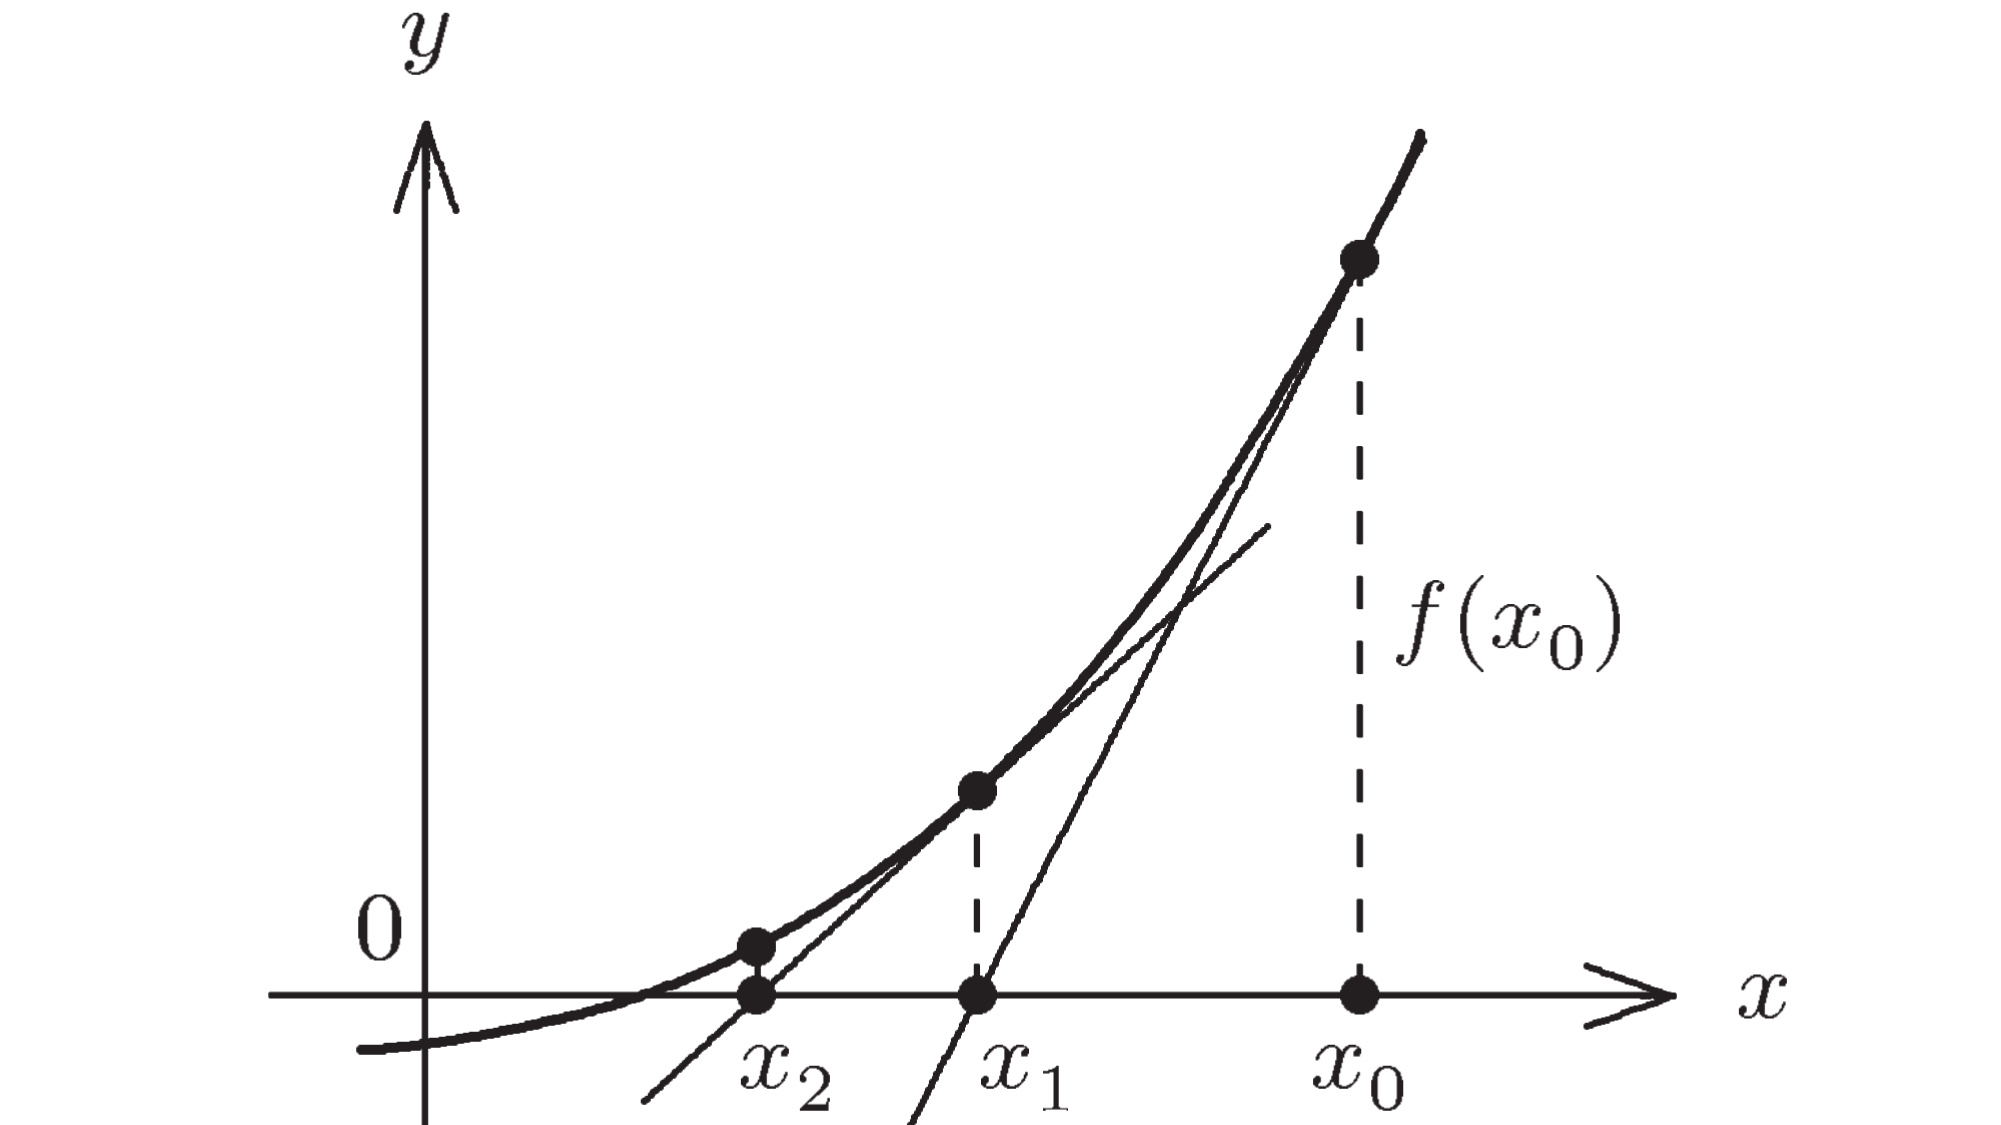
\includegraphics[width=3in]{Newton.jpg}
	\caption{$x_2$比$x_1$更好}
	\label{fig:wiki}
\end{figure}    
\end{frame}

\begin{frame}
\par 可以看出, 每次迭代其实是在$x_n$处将$f$看成其泰勒展开的一阶近似, 并求解此线性方程得到新的解$x_{n+1}$.
\par 因此, 不断重复此过程, 即不断地求
\begin{equation}
x_{n+1} = x_n - \frac{f(x_n)}{f'(x_n)}
\label{eq:newton}
\end{equation}
即可求得根的近似值.
\end{frame}

\begin{frame}
    \framesubtitle{算法流程图}
    \begin{figure}[htb]
        \centering
        \begin{tikzpicture}[node distance=10pt, hv path/.style = {to path={-| (\tikztotarget) \tikztonodes}}]
        \node[draw, rounded corners]						 (sstart)   {Start};
        \node[draw, rounded corners, below=of sstart]		 (start)	{给定$f, f'$和$x_0$};
        \node[draw, below=of start]							 (step 1)	{根据\ref{eq:newton}求出$x_1$};
        \node[draw, diamond, aspect=2, below=of step 1]		 (choice 1) {$|x_1 - x_0| < eps$};
        \node[draw, rounded corners, below=of choice 1]		 (end)		{end};
        \coordinate[right=30pt of step 1]					 (px);
        
        \graph{
            (sstart) -> (start) -> (step 1) -> (choice 1) -> ["Yes"left] (end);
        };
        \draw[rounded corners] (choice 1) -- node[above, near start] {No} (choice 1-|px) -> (px);
        \draw[->, rounded corners] (px) -- node[above, very near end] {$x_1$} (px|-start) -> (start);
        
        \end{tikzpicture}
        \caption{Newton法流程图}
        \label{fig:newton}
        \end{figure}
\end{frame}
%---

\begin{frame}
    \frametitle{数值算例}
    由上一节关于收敛速度的讨论, 可以知道Newton法在理论上比二分法收敛的更快一些. 下面通过一个高次多项式的例子来比较这两个算法实际上的好坏.
    $f(x) = 8x^5 + x^4 + 9x^2 + 7x + 5$
    \par \textbf{二分法:}设置初始区间为$[-e, 0], eps = 10^{-5}$, 则此算法表现如下:
\end{frame}

\begin{frame}
    \par \textbf{二分法:}设置初始区间为$[-e, 0], eps = 10^{-5}$, 则此算法表现如下:
\begin{table}[h]
    \small \scriptsize
    \begin{tabular}{lllll}
    iter & lower       & upper      & root       & err(est)  \\
    1    & -1.3591409, & 0.0000000  & -0.6795705 & 1.3591409 \\
    2    & -1.3591409, & -0.6795705 & -1.0193557 & 0.6795705 \\
    3    & -1.0193557, & -0.6795705 & -0.8494631 & 0.3397852 \\
    4    & -1.0193557, & -0.8494631 & -0.9344094 & 0.1698926 \\
    5    & -1.0193557, & -0.9344094 & -0.9768825 & 0.0849463 \\
    6    & -1.0193557, & -0.9768825 & -0.9981191 & 0.0424732 \\
    7    & -1.0193557, & -0.9981191 & -1.0087374 & 0.0212366 \\
    8    & -1.0087374, & -0.9981191 & -1.0034283 & 0.0106183 \\
    9    & -1.0034283, & -0.9981191 & -1.0007737 & 0.0053091 \\
    10   & -1.0007737, & -0.9981191 & -0.9994464 & 0.0026546 \\
    11   & -1.0007737, & -0.9994464 & -1.0001100 & 0.0013273 \\
    12   & -1.0001100, & -0.9994464 & -0.9997782 & 0.0006636 \\
    13   & -1.0001100, & -0.9997782 & -0.9999441 & 0.0003318 \\
    14   & -1.0001100, & -0.9999441 & -1.0000271 & 0.0001659 \\
    15   & -1.0000271, & -0.9999441 & -0.9999856 & 0.0000830 \\
    16   & -1.0000271, & -0.9999856 & -1.0000063 & 0.0000415 \\
    17   & -1.0000063, & -0.9999856 & -0.9999960 & 0.0000207 \\
    18   & -1.0000063, & -0.9999960 & -1.0000012 & 0.0000104 \\
    19   & -1.0000012, & -0.9999960 & -0.9999986 & 0.0000052
    \end{tabular}
    \end{table}

\par 二分法迭代19次后达到目标精度. \\
\end{frame}

\begin{frame}
    \par \textbf{牛顿迭代法:}设置初始点$x_0 = 0, eps = 10^{-5}$, 则此算法表现如下:
\newpage
\begin{table}[h]
    \begin{tabular}{lll}
    iter & root       & err(est)    \\
    1    & -0.7142857 & -0.7142857 \\
    2    & -1.8005532 & -1.0862675 \\
    3    & -1.4795259 & 0.3210273  \\
    4    & -1.2432980 & 0.2362280  \\
    5    & -1.0892808 & 0.1540172  \\
    6    & -1.0164491 & 0.0728317  \\
    7    & -1.0006718 & 0.0157774  \\
    8    & -1.0000012 & 0.0006706  \\
    9    & -1.0000000 & 0.0000012 
    \end{tabular}
    \end{table}
    \par 可以看到, 牛顿法迭代9次后即达到目标精度, 显著优于二分法.
\end{frame}

\begin{frame}
    \frametitle{二分法的函数图像}
    \begin{figure}[]
        \centering
        \begin{tikzpicture}
        \begin{axis}
        \addplot[domain=-1.5:-0.5, color=black]{8*x^5 + x^4 + 9*x^2 + 7*x + 5};
        \addplot[only marks, mark=square*, color=blue]
        coordinates{
            (-0.6795705,3.4531470)
            (-1.0193557,0.5088009)
            (-0.8494631,2.5302889)
            (-0.9344094,1.3808603)
            (-0.9768825,0.5441281)
            (-1.0087374,0.2234482)
            (-1.0034283,0.0864745)
            (-1.0007737,0.0193814)
            (-0.9994464,0.0138201)
            (-1.00011,0.0027508)
            (-0.9997782,0.0055418)
            (-0.9999441,0.0013973) 
            (-1.0000271,0.0006775)
            (-0.9999856,0.0003600)
            (-1.0000063,0.0001575)
            (-0.999996,0.0001000)
            (-1.0000012,0.0000300)
            (-0.9999986,0.0000350)
        };
        \end{axis}
        \end{tikzpicture}
        \caption{二分法}
        \end{figure}
\end{frame}
\begin{frame}
    \frametitle{牛顿迭代法的函数图像}
    \begin{figure}[]
        \centering
        \begin{tikzpicture}
        \begin{axis}
        \addplot[domain=-2:-0.5, color=black]{8*x^5 + x^4 + 9*x^2 + 7*x + 5};
        \addplot[only marks, mark=square*, color=red]
        coordinates{
            (-0.7142857,3.3646695)
            (-1.8005532,-119.3133087)
            (-1.4795259,-37.5796433)
            (-1.243298,-11.1680613)
            (-1.0892808,-2.8067487)
            (-1.0164491,-0.4291559)
            (-1.0006718,-0.0168244)
            (-1.0000012,0.0000300)
            (-1,0.0000000)
        };
        \end{axis}
        \end{tikzpicture}
        \caption{牛顿迭代法}
        \end{figure}
\end{frame}
%---

\begin{frame}
    \frametitle{分析}
    可以看出, 不管是理论上还是实际例子中, Newton法在求解函数的根问题上都优于二分法, 不过其有可导的前提, 在应用上没有二分法广泛。
\end{frame}

%---

\begin{frame}{参考文献}
	\printbibliography
    \nocite{zhihu144536388}
    \nocite{re1}
    \nocite{re2}
    \nocite{re3}
\end{frame}

\end{document}